\documentclass{ansarticle-preprint}
%\usepackage{ucs}
\usepackage[utf8]{inputenc}
\usepackage{amsmath}
%\usepackage{cite}
\usepackage{anslistings}

\usepackage{fontenc}
\usepackage{graphicx}

\hypersetup{
  pdfauthor={Wolfgang Bangerth, Timo Heister, Luca Heltai, Guido Kanschat,
    Martin Kronbichler, Matthias Maier, Bruno Turcksin
  %, Toby D. Young
  },
  pdftitle={The deal.II Library, Version 8.3, 2015},
}

\newcommand{\specialword}[1]{\texttt{#1}}
\newcommand{\dealii}{{\specialword{deal.II}}}
\newcommand{\pfrst}{{\specialword{p4est}}}
\newcommand{\trilinos}{{\specialword{Trilinos}}}
\newcommand{\aspect}{\specialword{Aspect}}
\newcommand{\petsc}{\specialword{PETSc}}
\newcommand{\cmake}{{\specialword{CMake}}}
\newcommand{\autoconf}{{\specialword{autoconf}}}

\title{The \dealii{} Library, Version 8.3}
\author[1]{Wolfgang Bangerth}
\affil[1]{Department of Mathematics, Texas A\&M University, College Station,
    TX 77843, USA,
    %\href{mailto:bangerth@math.tamu.edu}
    {\texttt{bangerth@math.tamu.edu}}}
\author[2]{Timo Heister}
\affil[2]{Mathematical Sciences,
O-110 Martin Hall.
Clemson University.
Clemson, SC 29634, USA,
%\href{mailto:heister@clemson.edu}
{\texttt{heister@clemson.edu}}}
\author[3]{Luca Heltai}
\affil[3]{SISSA - International School for Advanced Studies, Via
  Bonomea 265, 34136 Trieste, Italy,
  %\href{mailto:luca.heltai@sissa.it}
  {\texttt{luca.heltai@sissa.it}}}
\author[4]{Guido Kanschat}
\affil[4]{Interdisciplinary Center for Scientific Computing (IWR),
  Universität Heidelberg, Im Neuenheimer Feld 368, 69120 Heidelberg, Germany,
  %\href{mailto:kanschat@uni-heidelberg.de}
  {\texttt{kanschat@uni-heidelberg.de}}}
\author[5]{Martin Kronbichler}
\affil[5]{Institute for Computational Mechanics, Technische
  Universität München, Boltzmannstr.~15, 85748 Garching b. München,
  Germany,
  %\href{mailto:kronbichler@lnm.mw.tum.de}
  {\texttt{kronbichler@lnm.mw.tum.de}}}
\author[6]{Matthias Maier}
\affil[6]{School of Mathematics, University of Minnesota, 127 Vincent Hall,
  206 Church Street SE, Minneapolis, MN 55455, USA,
  %\href{mailto:matthias.maier@iwr.uni-heidelberg.de}
  {\texttt{msmaier@umn.edu}}}
\author[7]{Bruno Turcksin}
\affil[7]{Department of Mathematics, Texas A\&M University, College Station,
  TX 77843, USA,
  %\href{mailto:turcksin@math.tamu.edu}
  {\texttt{turcksin@math.tamu.edu}}}
%\author[8]{Toby~D.~Young}
%\affil[8]{Institute of Fundamental Technological Research of the Polish
%  Academy of Sciences, ul. Pawińskiego 5b, Warsaw 02-106, Poland,
%  %\href{mailto:tyoung@ippt.pan.pl}
%  {\texttt{tyoung@ippt.pan.pl}}}

\renewcommand{\labelitemi}{--}


\begin{document}
\maketitle

\begin{abstract}
  This paper provides an overview of the new features of the finite element
  library \dealii{} version 8.3.
\end{abstract}


\section{Overview}

\dealii{} version 8.3 was released August 1, 2015. This paper provides an
overview of the new features of this release and serves as a citable
reference for the \dealii{} software library version 8.3. \dealii{} is an
object-oriented finite element library used around the world in the
development of finite element solvers. It is available for free under the
GNU Lesser General Public License (LGPL) from the \dealii{} homepage at
\url{http://www.dealii.org/}.

The major changes of this release are:
\begin{itemize}
\item Improved handling of parallel distributed meshes, including a better
  numbering of cells on coarse meshes. For meshes with many coarse cells, the
  previous Cuthill-McKee numbering would lead to very skinny partitions if the
  processor number was similar to the number of Cuthill-McKee layers. Instead,
  a hierarchical concept inspired by the Morton numbering has been applied to
  define close cells in terms of mesh connectivity, see Fig.~\ref{fig:numbering}. This leads to much better
  volume-to-surface ratios independently of the number of processors and
  combines nicely with the partitioning of additional child cells generated by
  p4est \cite{p4est} and speeds up certain iterative solvers.
\begin{figure}
\centering
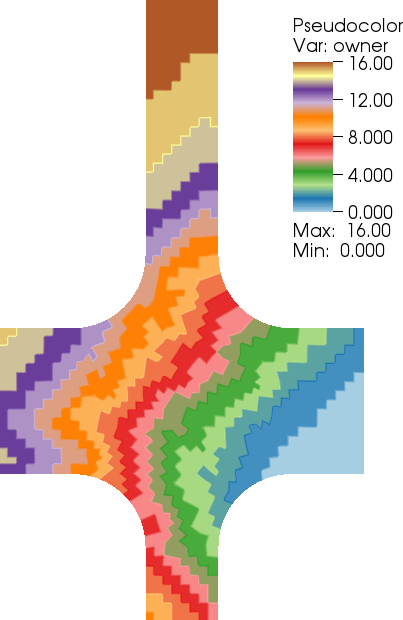
\includegraphics[height=6cm]{figures/83_cuthill_mckee_ordering.png}\quad
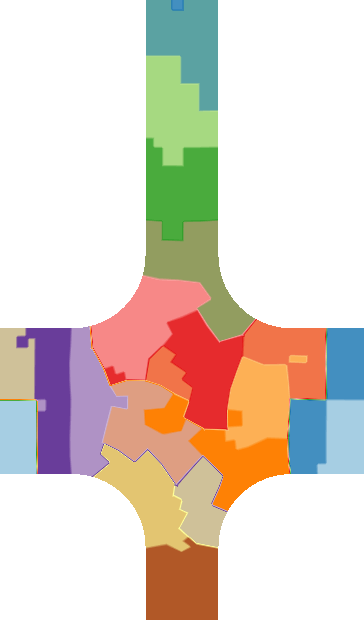
\includegraphics[height=6cm]{figures/83_hierarchical_ordering.png}
\caption{Comparison of old coarse-cell numbering by owner based on Cuthill-McKee (left) to the new hierarchical concept (right) on an unstructured mesh with 1100 elements on 17 MPI ranks.}
\label{fig:numbering}
\end{figure}
\item New abstract C++11 interface to linear operators.
\item All examples have been changed to use the new DynamicSparsityPattern.
\item Improved support for periodic boundary conditions with arbitrary
  orientations.
  %\item Initial support for isogeometric analysis.
\item New quadrature formulas.
\item Full conversion to the new manifold mechanism (manifold\_id) for boundary
  descriptions: \dealii{} previously utilized a mechanism in which one could
  ask ``boundary'' objects for new points on the boundary, but new points
  inside cells were always created by just averaging surrounding vertex
  locations. A previous version of \dealii{} introduced ``manifold'' objects
  for this, and they are now used consistently throughout the library.
\item Better support for complex-valued problems by doing internal arithmetic in
  the correct data types, rather than defaulting to double precision. In
  particular, we now correctly deduce and store the resulting type when
  multiplying pieces of data with different type (such as shape functions
  evaluated at quadrature points -- which are represented in \texttt{double}
  precision -- and the values of degrees of freedom -- which are represented
  in ways chosen by the user, including complex-valued data types).
\item An implementation of Bernstein polynomial-based finite elements.
\item Interface to the new algebraic multilevel package MueLu of the
  Trilinos project \cite{trilinos-web-page}.
\item More descriptive exception messages in many places for improved user
  productivity in code development.
\item  More than 140 other features and bugfixes.
\end{itemize}
Some of these will be detailed in the following section.
Information on how to cite \dealii{} is provided in Section \ref{sec:cite}.


\section{Significant changes to the library}

This release of \dealii{} contains a number of large and significant changes
that will be discussed in the following sections. It of course also contains a
vast number of smaller changes and added functionality; the details of these
can be found
\href{https://www.dealii.org/8.3.0/doxygen/deal.II/changes_between_8_2_1_and_8_3.html}{in the file that lists all changes for this release}
and that is linked to from the web site of each release as well as the
release announcement.


\subsection{Abstract concepts of linear operators}

\dealii{} now offers a versatile mechanism for storing the concept of a
linear operator as well as partially applied computations. The mechanism is
inspired by the \emph{expression template} optimization strategy, where C++
templates are used to create an arithmetic expression at compile time that can
then be efficiently be evaluated at runtime. In contrast to the template
approach, the implementation in \dealii{} utilizes C++11 features%
\footnotemark\footnotetext{Consequently, the classes outlined here are only
available in \dealii{} if the compiler in use supports C++11.}
such as \emph{lambda expressions} and \texttt{std::function} objects that
avoid the majority of the ``template overhead'' that usually comes with a
pure template solution. In particular, it avoids the often very lengthy and
cumbersome error messages associated with programming expression templates.

Our implementation only requires a minimal vector and matrix interface,
that all of \dealii's concrete vector and matrix types adhere to. For
example, in essence a matrix only has to provide a \texttt{vmult} method
for matrix-vector multiplication. This makes the interface fully
transparent with respect to the concrete matrix, or vector type that is
used, but naturally rules out further low-level optimization approaches
that can be used for non-distributed linear algebra (such as loop fusion).

The mechanism is centered around two classes, \texttt{LinearOperator} and
\texttt{PackagedOperation}. Both essentially consist of several
\texttt{std::function} objects that store the knowledge of how to apply a
linear operator, or a packaged operation, as well as how to initialize
vectors of range and domain space:
\begin{c++}
template <typename Range, typename Domain> class LinearOperator
{
public:
  std::function<void(Range &v, const Domain &u)> vmult;
  // ...
  std::function<void(Range &v, bool fast)> reinit_range_vector;
  std::function<void(Domain &v, bool fast)> reinit_domain_vector;
};

template <typename Range> class PackagedOperation
{
public:
  std::function<void(Range &v)> apply;
  // ...;
  std::function<void(Range &v, bool fast)> reinit_vector;
};
 \end{c++}

The primary purpose of the linear operator concept is to provide syntactic
sugar for complex matrix-vector operations and free the user from having to
create, set up, and handle intermediate storage locations by hand. As an
example, consider the operation $(A+k\,B)\,C$, where $A$, $B$ and $C$ denote
(possible different) matrices (or, in fact, other linear operators). In order
to construct a \verb|LinearOperator|
object \texttt{op} that encapsulates knowledge of this operation,
\dealii{} now allows one to write:

\begin{c++}
  dealii::SparseMatrix<double> A, B, C;
  const double k = ...;
  // Setup and assembly of matrices
  .
  const auto op_a = linear_operator(A);
  const auto op_b = linear_operator(B);
  const auto op_c = linear_operator(C);

  const auto op = (op_a + k * op_b) * op_c;
\end{c++}
Now, \texttt{op} can be used as a matrix object in its own right for
further computation. This includes passing it to any of \dealii{}'s linear
solver classes as the operator for which to solve a linear system. To make
this work, \dealii{} appropriately overloads arithmetic operators to allow
composition of linear operators as above.

The \texttt{PackagedOperation} class allows lazy evaluation of expressions
involving vectors and linear operators. This is done by storing the
computational expression and only performing the computation when either
the object is implicitly converted to a vector object, or if
\texttt{apply()} is invoked by hand. This avoids unnecessary temporary
storage of intermediate results. As an example consider the addition of
multiple vectors:
\begin{c++}
   dealii::Vector<double> a, b, c, d;
   // ..
   dealii::Vector<double> result = a + b - c + d;
\end{c++}

\texttt{operator+} (with two vector arguments) is implemented to return a
\texttt{PackagedOperation} whose \texttt{apply} function is implemented the
following way:
\begin{c++}
  apply = [&a, &b](Range &x) {
                                x = a;
                                x += b;
                             };
\end{c++}
Similarly, addition and subtraction of mixed vector and packaged operation
types are implemented. If implemented in the most straightforward way,
executing these additions would require the use of multiple temporary
vectors, along with the necessary memory allocation and de-allocation. On
the other hand, creating a \texttt{PackagedOperation} for the expression
\texttt{a + b - c + d} and converting it to a vector results in code
equivalent to the following:
\begin{c++}
   dealii::Vector<double> a, b, c, d;
   // ..
   dealii::Vector<double> result = a;
   result += b;
   result -= c;
   result += d;
\end{c++}
Consequently, this operation avoids the use of any intermediate storage.

Further, in addition to pure vector operations, scalar multiplication
(and thus all vector space operations) and application of a
\texttt{LinearOperator} to a vector can be expressed within a
\texttt{PackagedOperation}. For example, a residual can be expressed as:
\begin{c++}
  dealii::Vector<double> residual =  b - op_a * x;
\end{c++}
In all of these cases, \texttt{PackagedOperation} only stores references to
vector and linear operator arguments. As a consequence, creating a
\texttt{PackagedOperation} object and evaluating it multiple times will always
use the then-current values of the arguments, not the values at the time the
packaged operation was created.

\subsection{Initial support for iso-geometric analysis}

Nonuniform rational B-splines (NURBS) are the basis of most modern CAD packages.
Isogeometric analysis is a computational technique that aims at integrating
finite element analysis (FEA) into conventional NURBS-based CAD design
tools by directly using NURBS basis functions in
the FEA application~\cite{Cottrell2009}. The preliminary
implementation of the iso-geometric analysis concept in the \dealii{} library
is based on two main classes: a new finite element based on Bernstein
polynomials called \verb|FE_Bernstein| and a general mapping called
\verb|MappingFEField|, which generalizes the iso-parametric model to allow
the description of the geometry using arbitrary finite element displacement or
location fields.

The scalar Bernstein finite element \verb|FE_Bernstein|, in analogy
with \verb|FE_Q|, yields the finite element space of continuous,
piecewise Bernstein polynomials of degree $p$ in each coordinate
direction~\cite{Cottrell2009}. This class is realized using tensor
product polynomials of Bernstein basis polynomials.

The \verb|MappingFEField| is a generalization of the
\verb|MappingQEulerian| class, for arbitrary vector finite elements. The
two main notable differences are that this class interprets the degrees of
freedom of the underlying \verb|DoFHandler| as absolute positions
instead of displacements; and it
allows for arbitrary finite element types.
This class effectively decouples topology from geometry, by relegating all
geometrical information to the components of a FiniteElement vector field.
The underlying \verb|Triangulation| class is only used to infer topological
and connectivity information between cells.

(This feature was primarily developed by Marco Tezzele.)


\subsection{New quadrature formulas}

Two specialized quadrature formulas have been added to the library.

\subsubsection{Telles quadrature formulas}

Many applications require the integration of functions which might be
singular in some a-priori known point locations. A common strategy in such
cases, which was already implemented in the library, is the use of
Lachat-Watson quadrature formulas~\cite{Lachat1976}. These formulas are
fairly accurate but very expensive. A new quadrature formula for singular
integrals was introduced in \dealii{} that implements the quadrature formula
developed by Telles in~\cite{Telles-2005-a}.

The main idea of this quadrature formula is to create an iso-morphism of a
standard Gauss quadrature formula according to a nonlinear transformation
that has both first and second order derivatives equal to zero at the
singularity point.  Such a transformation removes the singularity of the
integrand and drops the approximation error from about the $10 \%$ to
$0.3\%$ for a large class of singular integrands~\cite{Telles-2005-a}. These
quadrature formulas are particularly relevant for approximation of Boundary
Integral Equations (see, e.g.,~\cite{GiulianiMolaHeltai-2015-a}).

(This feature was primarily developed by Nicola Giuliani.)


\subsubsection{Gauss-Chebyshev quadrature formulas}

Gauss-Chebyshev quadrature formulas~\cite{AbramowitzStegun} are used to
approximate integrals of functions on the interval $[-1,1]$ with weight
$w(x)=(1-x^2)^{-1/2}$.  In \dealii{} the reference interval is $[0,1]$, hence
our implementation of Gauss-Chebyshev formulas are mapped to this interval,
and the weight is changed to $w(x)=1/\sqrt{x(1-x)}$.

As for the other Gaussian quadrature formulas, three flavors of
Gauss-Chebyshev quadrature rules have been implemented for any order:
\begin{description}
\item[Gauss-Chebyshev (GC)] formulas with $N$ points that integrate
  exactly polynomials up to the order $2N-1$;
\item[Gauss-Radau-Chebyshev (GRC)] formulas with $N$ points where one of
  the two endpoints of the interval can be specified as a constrained
  quadrature point; these formulas are exact up to the order $2N-2$;
\item[Gauss-Lobatto-Chebyshev (GLC)] formulas with $N$ points where two
  quadrature nodes are constrained to lie on the boundary points of the
  interval; these formulas exactly integrate polynomials up to the order $2N-3$.
\end{description}

One important application of the GLC quadrature formulas is in the context
of Spectral Element Methods (SEM) using Lagrangian interpolants on GLC
points as basis functions (this is a good choice for the composite
interpolation of ``very regular'' continuous functions). This pair of basis
functions and quadrature formulas generates diagonal mass matrices, that
can be efficiently applied both in direct and in inverse form. For saddle
point problems, one common choice in SEM~\cite{MadayPatera} is the
$\mathbb{Q}_N-\mathbb{Q}_{N-2}$ (inf-sup stable) couple based on Lagrangian
interpolants on $N+1$ GLC and $N-1$ GC nodes respectively.

(This feature was primarily developed by Giuseppe Pitton.)


\subsection{Better error messages}

\dealii{} uses assertions extensively to validate that input arguments to
functions are within their allowed ranges, are mutually consistent, and
satisfy appropriate preconditions. We also use assertions to check for
internal conditions as well as for postconditions of many functions. All told,
the sources of \dealii{} contain around 9,000 assertions.

Whenever an assertion is failed, \dealii{} aborts the program with an error
message that includes the failing condition, its location, the surrounding
function's name, the call stack, and additional information specific to the
exception class associated with this particular error. For example, trying to
read an element of a vector that does not exist would trigger the exception in
the following code:
\begin{c++}
template <typename Number>
inline
Number Vector<Number>::operator() (const size_type i) const
{
  Assert (i<vec_size, ExcIndexRange(i,0,vec_size));
  return val[i];
}
\end{c++}
The error message produced from this code would look like this:
\begin{verbatim}
--------------------------------------------------------
An error occurred in line <1222> of file <.../include/deal.II/lac/vector.h> in function
    Number& dealii::Vector<number>::operator()(dealii::Vector<number>::size_type)
      [with Number = double, dealii::Vector<number>::size_type = unsigned int]
The violated condition was:
    i<vec_size
The name and call sequence of the exception was:
    ExcIndexRangeType<size_type>(i,0,vec_size)
Additional Information:
Index 123456 is not in the half-open range [0,679).

Stacktrace:
-----------
#0  ./step-22: dealii::Vector<double>::operator()(unsigned int)
#1  ./step-22: Step22::StokesProblem<2>::assemble_system()
#2  ./step-22: Step22::StokesProblem<2>::run()
#3  ./step-22: main
--------------------------------------------------------
\end{verbatim}

In this case, the error message does state the index that is being accessed,
as well as the size of the vector, both under ``Additional Information''. The
error message may not be overly clear, but it helps illustrate the values of
variables that participated in the failed condition \verb|i<vec_size|.

However, many error messages produced by \dealii{} either do not produce any
additional information at all, or very little that is understandable to a
novice user. Observing users deal with errors in the courses we teach has
shown that poor error messages are a major obstacle to quickly identifying the
causes of problems. Ideally, error messages would attempt to explain what is
going wrong, what are typical causes for this, and what possible solutions
are.

In an effort to improve this situation, we have rewritten and augmented the
error messages produced by several dozen classes of assertions. Going through
the remainder of all error messages is a longer-term project.


\subsection{Incompatible changes}

This version of \dealii{} contains a number of changes that are
incompatible with previous versions. A complete list can be found
\href{https://www.dealii.org/8.3.0/doxygen/deal.II/changes_between_8_2_1_and_8_3.html}{in
  the file that lists all changes for this release}. Most of these
changes are corner cases that are not likely to affect a
significant fraction of users. In particular, many of these changes
remove functions and classes that were already deprecated (and
produced a compiler warning); often these functions had been marked as
depracted for several years already.

The only change that has the potential to be of more general interest
is a clarification of the \texttt{Tensor<1,dim>} and
\texttt{Point<dim>} classes. As they both represent vectors in a
\texttt{dim}-dimensional space, they were previously often used
interchangeably. This has been changed in many places where we
semantically now associate \texttt{Point<dim>} with a \textit{point}
in space, i.e., a vector anchored at the origin; and where we
semantically associate \texttt{Tensor<1,dim>} with vectors anchored
anywhere.

An example is that \texttt{operator-(Point<dim>, Point<dim>)} now
returns a \texttt{Tensor<1,dim>}. Likewise, normal vectors to cells
are also represented by this latter data type. Overall, there are few
resulting incompatibilities, with the exception being assigning an
expression that previously was a \texttt{Point<dim>} but now is a
\texttt{Tensor<1,dim>} (such as the difference between two points) to
a variable of type \texttt{Point<dim>}. In most contexts, however,
everything will continue to work because a \texttt{Point<dim>} can
automatically be (down-)cast to a \texttt{Tensor<1,dim>}.


\section{How to cite \dealii{}}\label{sec:cite}

In order to justify the work the developers of \dealii{} put into this
software, we ask that papers using the library reference one of the
\dealii{} papers. This helps us justify the effort we put into it.

There are various ways to reference \dealii{}. To acknowledge the use of a
particular version of the library, reference the present document. For up
to date information and bibtex snippets for this document see:

\bigskip

\begin{center}
 \url{https://www.dealii.org/publications.html}
\end{center}

\bigskip

% \begin{minipage}{0.9\textwidth}%no page break in here please
% \begin{verbatim}
% @article{dealII82,
%   title = {The {\tt deal.{I}{I}} Library, Version 8.2},
%   author = {W. Bangerth and T. Heister and L. Heltai
%    and G. Kanschat and M. Kronbichler and M. Maier
%    and B. Turcksin and T. D. Young},
%   journal = {preprint},
%   year = {2015},
% }
% \end{verbatim} %  journal = {arXiv preprint \url{http://arxiv.org/abs/TODO}},
% \end{minipage}

The original \texttt{\dealii{}} paper containing an overview of its
architecture is \cite{BangerthHartmannKanschat2007}. If you rely on specific
features of the library, please consider citing any of the following:
\begin{itemize}
 \item For geometric multigrid: \cite{Kanschat2004,JanssenKanschat2011};
 \item For distributed parallel computing: \cite{BangerthBursteddeHeisterKronbichler11};
 \item For $hp$ adaptivity: \cite{BangerthKayserHerold2007};
 \item For matrix-free and fast assembly techniques:
   \cite{KronbichlerKormann2012};
 \item For computations on lower-dimensional manifolds:
   \cite{DeSimoneHeltaiManigrasso2009};
 \item For integration with CAD files and tools:
   \cite{HeltaiMola2015};
 \item For \texttt{LinearOperator} and \texttt{PackagedOperation} facilities:
   \cite{MaierBardelloniHeltai-2015-a}.
\end{itemize}

\dealii{} can interface with many other libraries:
\begin{itemize}
\item ARPACK \cite{arpack}
\item BLAS, LAPACK
\item HDF5 \cite{hdf5}
\item METIS \cite{karypis1998fast}
\item MUMPS \cite{ADE00,MUMPS:1,MUMPS:2,mumps-web-page}
\item muparser \cite{muparser-web-page}
\item NetCDF \cite{rew1990netcdf}
\item OpenCASCADE \cite{opencascade-web-page}
\item p4est \cite{p4est}
\item PETSc \cite{petsc-user-ref,petsc-web-page}
\item SLEPc \cite{Hernandez:2005:SSF}
\item Threading Building Blocks \cite{Rei07}
\item Trilinos \cite{trilinos,trilinos-web-page}
\item UMFPACK \cite{umfpack}
\end{itemize}
Please consider citing the appropriate references if you use interfaces to these
libraries.

Older releases of \dealii{} can be cited as \cite{dealII80,dealII81,dealII82}.

\nocite{BangerthKanschat1999}

\section{Acknowledgments}

\dealii{} is a world-wide project with dozens of contributors around the
globe. Other than the authors of this paper, the following people contributed code to
this release:
%
% get this from the changes.h file using
%   egrep '^ *\(.*2015' 8.2.1-vs-8.3.0.h | perl -p -e 's/2015.*//g; s/,/\n/g; s/^ *\(?//g;' | sort | uniq
% then sort by last name and remove the authors of this paper
%
Daniel Arndt,
Mauro Bardelloni,
Praveen C,
Denis Davydov,
Anton Evgrafov,
Arezou Ghesmati,
Nicola Giuliani,
Lukas Korous,
Ross Kynch,
Giuseppe Pitton,
Fernando Posada,
Lei Qiao,
Angel Rodriguez,
Ian Rose,
Florian Sonner,
Martin Steigemann,
Zhen Tao,
Marco Tezzele,
David Wells.

Their contributions are much appreciated!


\dealii{} and its developers are financially supported through a
variety of funding sources. W.~Bangerth and B.~Turcksin were partially
supported by the National Science Foundation under award OCI-1148116
as part of the Software Infrastructure for Sustained Innovation (SI2)
program; and by the Computational Infrastructure in Geodynamics initiative
(CIG), through the National Science Foundation under Award
No.~EAR-0949446 and The University of California -- Davis.

L.~Heltai was partially supported by the project OpenViewSHIP,
``Sviluppo di un ecosistema computazionale per la progettazione
idrodinamica del sistema elica-carena'', financed by Regione FVG - PAR
FSC 2007-2013, Fondo per lo Sviluppo e la Coesione, and by the project
TRIM ``Tecnologia e Ricerca Industriale per la Mobilit\`a Marina'',
CTN01-00176-163601, funded by MIUR -  Ministero dell'Istruzione,
dell'Universit\`a e della Ricerca.

T.~Heister was partially supported by the Computational Infrastructure in
Geodynamics initiative (CIG), through the National Science Foundation under Award
No. EAR-0949446 and The University of California -- Davis.

The Interdisciplinary Center for Scientific Computing (IWR) at Heidelberg University has provided
hosting services for the \dealii{} web page and the SVN archive.

%\marginpar{Everyone's funding, please}


\bibliography{deal83}{}
\bibliographystyle{abbrv}

\end{document}
